\chapter{Integration Design and Architecture}
\label{cha:integration_design_and_architecture}

This chapter presents the design of the solution developed in this work to connect Legion clients to the Antidote data storage. We start by briefly presenting Antidote and Legion, focusing on the mechanisms necessary for integrating both systems. After this introduction, we presents an overview of the proposed design and the interaction between Legion and Antidote.

\section{Overview of used systems}
\label{sec:system_introduction}
In order to design an integration between Legion and Antidote, it is imperative that we understand how both systems work, so we can take advantage of their internal mechanisms. Next follows a brief presentation of the mentioned systems, as well as some important working details.

\subsection{Legion}
\label{sec:legion_intro}
A large number of web application are built around direct interactions among clients, such as collaborative applications, social networks and multi-user games. These applications manage a set of shared objects, with each user reading and writing to a subset of these objects. These kind of applications are usually implemented using a centralized infrastructure that maintains the shared state and mediates all interactions among users. This approach has some drawbacks, such as the servers becoming a scalability bottleneck, the service interrupt when the servers are unavailable and the latency for nearby users being unnecessarily high.\par
	One alternative to this model, is to rely on direct communication between users. In a not so far past, such an alternative would be troublesome when combining peer-to-peer and to rely on Web applications. Due to the lack of default mechanisms for supporting peer-to-peer communications, it was often needed browser extensions or plugins to implement such approach.\par
	With the recent development of tools such as WebRTC\cite{webrtc}, that enables direct communication between browsers and connectivity utilities such as STUN and TURN, as explained in \ref{sec:webrtc}, that can overcome the trouble of connecting users behind NATs and firewalls, a new set of peer-to-peer web applications started to be developed.\par
	Legion is a framework that exploits these new features for enriching web applications with direct data replication between browsers. Each client maintains a local data storage with replicas of a subset of application shared objects. Legion uses an eventual consistency model, where each client can modify its local objects without coordination. This allows updates to be performed concurrently on different replicas, with modifications being propagated asynchronously. To guarantee that all replicas converge to the same correct state after updates have been applied in different replicas, Legion relies on CRDTs\cite{crdt} for representing data. To support interactions in a peer-to-peer manner, clients form overlay networks to propagate objects and updates among them. In each overlay network, a few clients act as synchronization points with a centralized component, that acts as a centralized persistent storage. These clients have an object server component that include an extension mechanism to allow the integration with different central services. These clients are responsible to propagate updates executed in the Legion overlay to the central service and vice-versa. Figure \ref{legion_architecture} illustrates the Legion's architecture.
	
\begin{figure}[H]
\centering
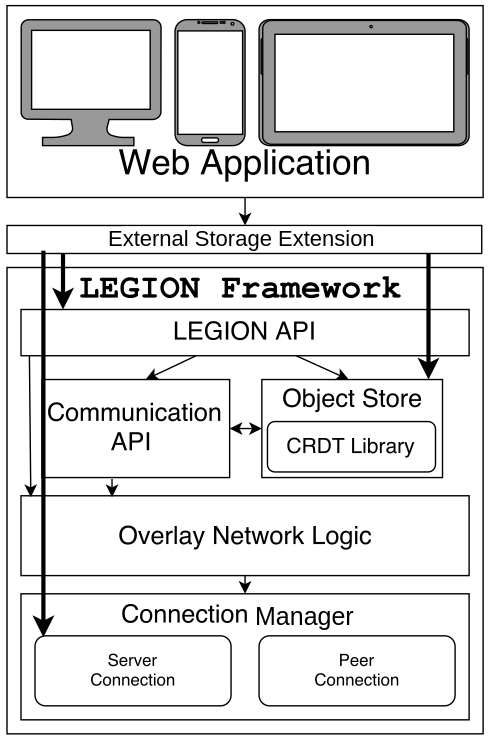
\includegraphics[scale=0.3]{files/legionArchitecture.png}
\caption{Legion Architecture}
\label{legion_architecture}
\end{figure}

\subsection{Antidote}
\label{sec:antidote_intro}
Traditional databases, as discussed in \ref{sec:relational_model}, provide strong guarantees but are slow and unavailable under failures and network partition. Hence, they are not suitable for geo-replication. The alternatives are NoSQL-style databases which are fast and available even under network partition. As described in \ref{sec:key-value_model}, they provide a low-level key-value interface and expose data inconsistencies due to asynchronous communication among the servers. It takes significant effort and expertise from programmers to deal with these inconsistencies and develop correct applications on top of these databases. Antidote\cite{site_antidote} provides features that aid programmers to write correct applications, while having the same performance and horizontal scalability as NoSQL, from a single machine to geo-replicated deployments, with the added guarantees of Causal Highly-Available Transactions, and provable absence of data corruption due to concurrency.\par
	Internally, Antidote uses CRDTs to store data. To modify the database, one can make use of interactive transactions composed by three steps: begin, update/read and finally commit. Transactions can receive a timestamp to force the read/update to be executed at a certain system snapshot. Antidote low-level API allows to request the operations log since a certain timestamp. Clients can use this API via the distributed Erlang interface that can only be used by Erlang clients, or the protocol buffer interface\cite{protocol_buffers}, which is language independent. Antidote can work with several nodes in the same cluster, and the inter-dc mode replicates data in a FIFO (First in first out) operation order. The system architecture is depicted in figure \ref{antidote_architecture}.

\begin{figure}[H]
\centering
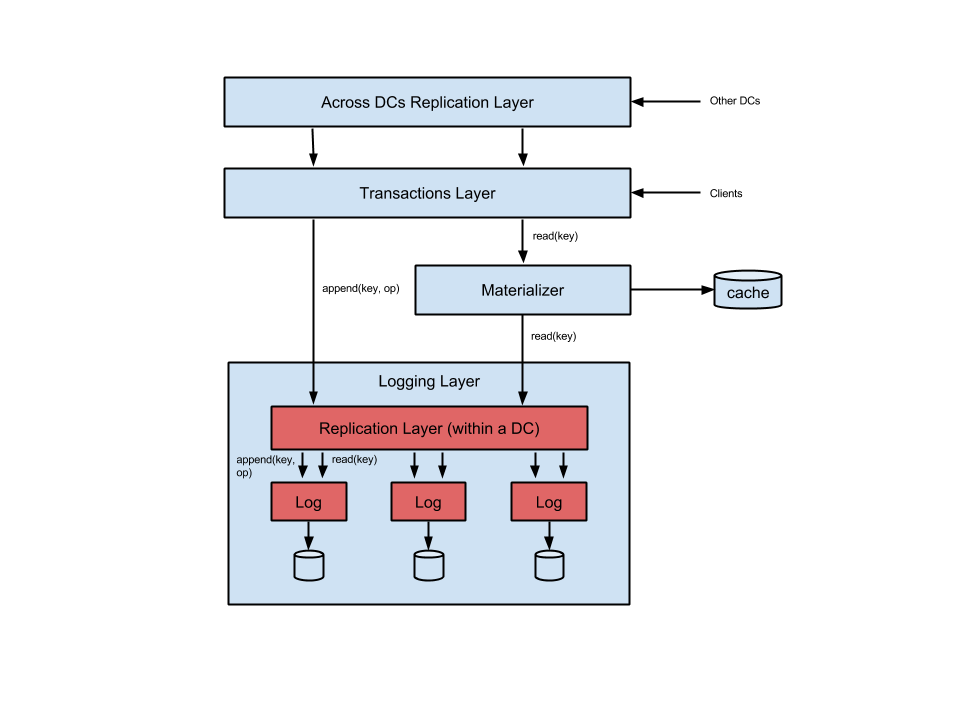
\includegraphics[scale=0.4]{files/antidoteArchitecture.png}
\caption{Antidote Architecture}
\label{antidote_architecture}
\end{figure}

\section{Architecture Overview}
\label{sec:architecture_overview}
Legion includes a mechanism to allow the integration with other external storage systems, which we use in our work. This mechanism consists in a module that implements a pre-defined interface.\par
	Figure \ref{architecture} shows the architecture of our approach to integrate Legion with Antidote.
	
\begin{figure}[h]
\centering
\includegraphics[scale=0.5]{files/architecture.png}
\caption{Integration Architecture}
\label{architecture}
\end{figure}

\par
	The following components are included in the architecture.
\begin{description}

\item[Antidote] \hfill \\
The storage system to be integrated with Legion. Antidote is a geo-replicated data store with servers running in multiple DCs. The replicas in Antidote will be synchronized with Legion. An Antidote node can have its data updated directly by an antidote client, or by an update that was propagated by a Legion node.\par

\item[Antidote Client] \hfill \\
An Antidote client can manipulate the system's data by making calls to modify the state of Antidote's objects directly.\par
	An Antidote client can be any client that either uses Antidote's distributed Erlang interface, or the protocol buffer interface.


\item[Legion Node] \hfill \\
This component is a Legion instance in the system. Applications running in Legion nodes can query and update data in the system. Legion nodes also have the responsibility to keep themselves and the other Legion nodes updated and synchronized.


\item[Legion's Objects Server] \hfill \\
The objects server is part of a legion node and acts as a synchronization point to centralized storages. There can be one or more in each Legion network, and it is guaranteed that every event in the Legion network will be captured by at least one objects server. These events include network membership messages and update operations. In our work, the objects server sends updates to Antidote using the protocol buffer interface. The objects server gets operations from Antidote and feeds them into the Legion network.\par
	As we will detail later, this component communicates with the ZooKeeper service to coordinate their execution.

\item[ZooKeeper Service] \hfill \\
ZooKeeper is used in the system as a service to guarantee mutual exclusion of the synchronization process between the multiple objects servers. It receives locking requests from Legion's objects servers and keeps information of the locking status of each data object.

\end{description}

\section{Integration challenges}
\label{sec:integration_challenges}
When integrating both systems, there are some challenges that need to be tackled. The main effort in this integration is the synchronization process, which must be executed by propagating operations from one system to another. CRDTs internally store metadata used to guarantee that replicas converge to the same state after all updates are executed. This metadata is also included in the operations. However, as Antidote and Legion use slightly different information, it is necessary to convert the metadata when operations are propagated across systems. For example, when an element is inserted to a set in Legion, a unique identifier composed by the node id and a counter is associated with the element. When an operation is sent to Antidote, it is necessary to convert this unique identifier in one of the identifiers used in Antidote. The same occurs when an operation is propagated from Antidote to Legion.\par
	Despite multiple Legion object servers may contact Antidote, we need to guarantee that an operation executed in Legion (respectively Antidote) generates a single operation in Antidote (respectively Legion). To achieve this, we use the following approach.\par
	First, we need to guarantee that a single object server is synchronizing at any given moment. To this end we use ZooKeeper to guarantee the mutual exclusion between objects servers.\par
	Second, we record in Antidote the mapping of metadata used in operations between Legion and Antidote. Additionally, each Legion network always contacts the same Antidote DC, which guarantees that the mappings will be available. With these mappings, the operations created by objects servers will be identical and idempotent. We note that it is necessary to allow different objects servers to propagate the same operation from Antidote to Legion, as a node running the objects server may fail before propagating the received operation to other nodes.\par
	The solution of these challenges is described in sections \ref{sec:legion_to_antidote_flow} and \ref{sec:antidote_to_legion_flow}, by explaining step by step how the data is propagated between systems, keeping the system's objects synchronized along with the related metadata.

\section{Legion to Antidote flow}
\label{sec:legion_to_antidote_flow}
This section details the process of propagating an update issued by a Legion node into Antidote, which is presented in Algorithm \ref{legion_to_antidote_algorithm}.\par
	In order to send the updates from Legion to Antidote we must first detect these updates. Since every update issued by a Legion node is propagated to at least one of the objects servers, we implement this process in the objects server. Our algorithm processes each event that occurs in he objects server. If the event is an update, it will be checked if that operation was already propagated to Antidote, since more than one objects server can exist. If it was not, the operation is propagated in a transaction that adds the Legion ID of he operation to the set of operations done, and executes he correspondent operation in the Antidote object. This process is executed in mutual exclusion, enforced by using ZooKeeper to guarantee that a Legion operation only generates a single Antidote operation.
	
\begin{algorithm}
\caption{Legion to Antidote flow}
\label{legion_to_antidote_algorithm}
\begin{algorithmic}[1]
\algblock{Upon}{End}
\Upon { $event$:}
  \If {$event.type$ = $update$}
    \State {objectsServer.apply($update$)}
    \State {$metaData$ $\gets$ parse($update$)}
    \State {$doneOperation$ $\gets$ antidote.read($doneOperations$)}
    \If {!($update.id$ in $doneOperations$)}
      \State {zooKeeper.lock($metadata.objectId$)}
      \State {antidote.write($metadata$)}
      \State {zooKeeper.unlock($metadata.objectId$)}
      \State {antidote.write($update.operations, lastSeenTimestamp$)}
      \State {return}
    \EndIf
  \EndIf
\End
\end{algorithmic}
\end{algorithm}

\section{Antidote to Legion flow}
\label{sec:antidote_to_legion_flow}
This section explains the process of propagating an update issued by an Antidote client into Legion. Algorithm \ref{antidote_to_legion_algorithm} shows this process step by step.\par
	For an Antidote client to issue an update, it makes use of the protocol buffer interface\cite{protocol_buffers} to apply changes to the state of Antidote's objects. This operation is recorded in Antidote's log.\par
	The Legion objects servers are responsible for extracting new operations from Antidote and propagate them to the Legion network.Currently there are two mechanisms for sending the updates to the objects servers. It can be done using the internal public/subscribe system that fires an event every time an Antidote object is updated. This solution has one major problem. The update propagation mechanism would not handle lost messages, which would have to be handled by our system.
	Another method to achieve this, is to have Legion's objects servers probe Antidote periodically for new updates. This can be done using Antidote's operation log. Legion's objects servers will periodically make a request to get Antidote's operation log. This log contains the operations executed in Antidote since the objects server last seen snapshot. If there are no new updates, then the objects server only updates its last seen timestamp. If there are new updates that were not propagated to Legion, the objects server executes the operation locally, and then propagates it through the Legion network. The objects server also needs to update the related meta-data for each object in the update.
	
\begin{algorithm}
\caption{Antidote to Legion flow}
\label{antidote_to_legion_algorithm}
\begin{algorithmic}[1]
  \algblock{Every}{End}
  \Every { 2 seconds:}
  \State {$logOperations$ $\gets$ antidote.get($logOperations$, $lastSeenTimeStamp$)}
    \ForEach {$operation \in logOperations$}
      \If {!($operation.id$ in objectsServer.$doneOperations$)}
        \State {$metadata$ $\gets$ parse($operation$)}
        \State {zooKeeper.lock($metadata.objectId$)}
        \State {antidote.write($metadata$)}
        \State {zooKeeper.unlock($metadata.objectId$)}
        \State {objectsServer.Apply($operation$)}
        \State {legion.Propagate($operation$)}
      \EndIf
    \EndFor
    \State {objectsServer.update($lastSeenTimestamp$)}
    \State {return}
  \End
\end{algorithmic}
\end{algorithm}